\documentclass[t]{beamer}

%\documentclass[handout, t]{beamer}
\setbeamertemplate{navigation symbols}{}
\usepackage{pstricks}
\usepackage{mathtools}
\usepackage{amsfonts}
\usepackage{mathrsfs}
\usepackage{amsmath}
\setbeamertemplate{navigation symbols}{}
\usepackage{bm}
\usepackage[UTF8]{ctex}
\usetheme{AnnArbor}
\usefonttheme{serif}
\useinnertheme{rounded}
\usecolortheme{beaver}
\setbeamertemplate{blocks}[rounded][shadow=true]

\newcommand{\dif}{{\;\rm d}}
\usepackage{graphicx}
\usepackage{pgf}
\usepackage{tikz}
\usetikzlibrary{arrows, decorations.pathmorphing, backgrounds, positioning, fit, petri, automata}
\tikzset{>=stealth}

\usepackage{setspace}
\setmainfont{Times New Roman}
\setCJKmainfont{Microsoft YaHei}
% \setCJKmainfont{苹方}   % 使用苹果MAC系统,请使用这个选项,并将上面的命令用%注释掉

\hypersetup{pdfpagemode=FullScreen}
\renewcommand{\Pr}{\mathbb{P}}
\usepackage{blkarray}


\setbeamercolor{block title}{bg=red!10!white}
\setbeamercolor{block body}{bg=gray!10!white}

\usepackage{multicol}
\newcommand{\E}{\mathbb{E}}
\newcommand{\EP}{\mathbb{E}^{\mathbb{P}}}
\newcommand{\EQ}{\mathbb{E}^{\mathbb{Q}}}
\newcommand{\Var}{{\rm Var}}
\newcommand{\Cov}{{\rm Cov}}
\usepackage{tkz-euclide}

\begin{document}
\fontsize{11}{18}\selectfont


\CTEXindent



  \title{第三章~~鞅}
\author{金融数学}
\date{中国人民大学出版社}
  \begin{frame}
    \maketitle
  \end{frame}

  \begin{frame}{鞅的起源}
    鞅(martingale)的概念最早起源于赌博中的双倍押注法(double gambling),
    在该策略下,如果每次输了就把下注的资金翻倍。对于公平赌博而言,如此反复最终总能赢钱。
    
    而在马术上,鞅指的是套在马颈上的缰绳(也称马颔缰),以防止马甩头,并借此控制马的行进方向。
    \begin{center}
    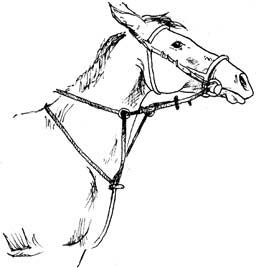
\includegraphics[scale=0.7]{fig/martingale.jpg}
    \end{center}
    
    \end{frame}
    
    
    \begin{frame}{鞅的应用}
    鞅(martingale)是一类重要的随机过程。
    鞅的研究丰富了概率论的内容,很多以往被认为是复杂的东西,在纳入鞅论的框架后得以简化。
    
    近几十年来,鞅理论不仅在随机过程中占据重要的地位,而且在金融、保险等领域的实际问题中得到了广泛的应用。
    \end{frame}
    
    \begin{frame}{相关学者}
    \centering
    \begin{tabular}{ccc}
    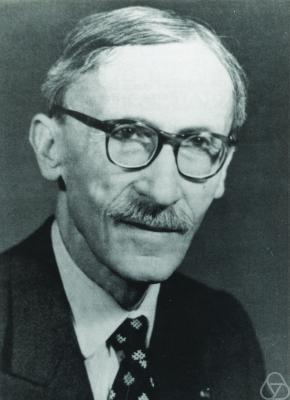
\includegraphics[height=.5\textheight]{fig/levy.jpg}&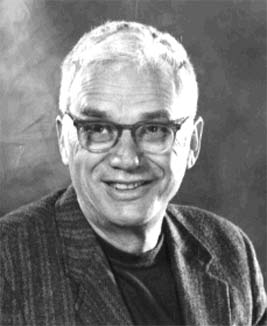
\includegraphics[height=.5\textheight]{fig/Doob.jpeg}&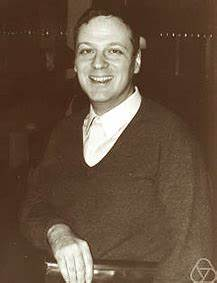
\includegraphics[height=.5\textheight]{fig/meyer.jpg}\\
    Paul P. Levy&Joseph L. Doob&Paul-Andr\'{e} Meyer\\
    1886--1971&1910--2004& 1934--2003\\
    \end{tabular}
    
    \end{frame}
    
    \begin{frame}{本章内容}
      \begin{multicols*}{2}
        \tableofcontents
      \end{multicols*}
      
      \end{frame}

      \section{条件期望}

      \begin{frame}{条件期望的概念}
      假设有两个随机变量$X$和$Y$,并且它们的取值取决于$N$次发生的事件构成的信息集$\{Z_1,Z_2,\ldots,Z_N\}$。以其中$n$次事件的信息集为条件,得到的随机变量期望就是条件期望(conditional expectation)。记作:
      \begin{equation*}
      \E_n(X)=\E(X|Z_1,Z_2,\ldots,Z_n),\quad \E_n(Y)=\E(Y|Z_1,Z_2,\ldots,Z_n)
      \end{equation*}
      \end{frame}
      
      \begin{frame}{可测的概念}
      随机变量$\E_n(X)$的值,仅与$Z_1,Z_2,\ldots,Z_n$有关时,可以将其写作
      \begin{equation*}
      \E_n(X)=\E(X|Z_1,Z_2,\ldots,Z_n)=f(Z_1,Z_2,\ldots,Z_n)
      \end{equation*}
      其中$f(\cdot)$是函数。显然此处随机变量$\E_n(X)$可以表示为$Z_1,Z_2,\ldots,Z_n$的函数,称$\E_n(X)$关于$Z_1,Z_2,\ldots,Z_n$可测(measurable)。
      \end{frame}
      
      \begin{frame}{条件期望的性质}
      \begin{itemize}
      \item 线性性质(linearity):对于所有常数$c_1$和$c_2$,以下等式成立:
      \[\E_n(c_1 X+c_2 Y)=c_1\E_n(X)+c_2\E_n(Y) \]
      \item 提取已知量(taking out what is known):若$X$的取值只依赖于$n$次事件的信息集,则:
      \[\E_n(XY)=X\cdot \E_n(Y) \]
      在这里,$X$在$n$次事件的信息集下是可测的,从而可以从条件期望中提取出来。
      \end{itemize}
      \end{frame}
      
      \begin{frame}{条件期望的性质(cont.)}
      \begin{itemize}
      \item 累次条件期望(iterated conditioning):若$0\le n\le m\le N$,则有:
      \[\E_n\left[\E_m(X)\right]=\E_n(X) \]
      从中可以看出,$X$的条件期望,取决于信息集中最小者。特别是针对无条件期望而言,有:
      \[\E\left[\E_m(X)\right]=\E(X) \]
      
      \item 独立性(independence):若$X$取决于第$(n+1)$到$N$次事件所构成的信息集$\{Z_{n+1},Z_{n+2},\ldots,Z_N\}$,则有:
      \[\E_n(X)=\E(X) \]
      因为此处的条件与随机变量$X$无关。
      \end{itemize}
      \end{frame}
      
      \begin{frame}{条件期望的性质(cont.)}
      
      \begin{itemize}
      \item 詹森(Jensen)不等式:
      如果$\phi(\cdot)$是凸函数,则下列不等式成立
      \begin{equation*}
      \E_n[\phi(X)]\ge \phi(\E_n(X))
      \end{equation*}
      \end{itemize}
      
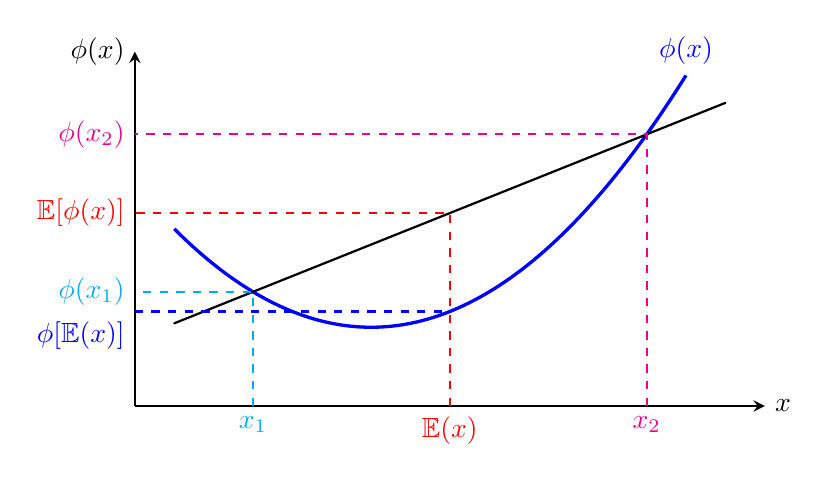
\begin{tikzpicture}[>=stealth, thick]
	\draw[->](0,0)--(0,4.5)node[left]{$\phi(x)$};
	\draw[->](0,0)--(8,0)node[right]{$x$};

\draw[domain=0.5:7, samples=100, color=blue, very thick] plot(\x, {0.2*(\x-3)*(\x-3)+1})node[above]{$\color{blue}\phi(x)$};

\tkzDefPoints{1.5/1.45/A, 6.5/3.45/B}

\tkzDrawLines[thick](A,B)
\draw[dashed, color=cyan](1.5,0)node[below]{$\color{cyan}x_1$}--(A)--(0,1.45)node[left]{$\color{cyan}\phi(x_1)$};
\draw[dashed, color=magenta](6.5,0)node[below]{$\color{magenta}x_2$}--(B)--(0,3.45)node[left]{$\color{magenta}\phi(x_2)$};
\draw[dashed, color=red](4,0)node[below]{$\E(x)$}--(4,2.45)--(0,2.45)node[left]{$\color{red}\E[\phi(x)]$};

\draw[dashed, color=blue](0,1.2)node[below left]{$\color{blue}\phi[\E(x)]$}--(4,1.2);



\end{tikzpicture}
      
     
      \end{frame}
      
      \section{鞅的概念和性质}
      
      \subsection{离散鞅}
      \begin{frame}{离散鞅的概念}
      
      假设有一个随机序列$\{X_n\},\; n=0,1,2,\ldots$,若对$\forall n\ge 0$,均有$\E|X_n|<\infty$,并且
      \begin{equation*}
      \E(X_{n+1}|X_n,\ldots, X_2, X_1)=X_n
      \end{equation*}
      则称$\{X_n\}$为离散鞅(discrete martingale)序列。	
      
      \begin{block}{注意:}
      离散鞅具有某种无后效性,并且随机变量$X_{n+1}$对之前所有信息下的条件期望,只取决于$n$时刻的$X_n$,而与$n$时刻之前的随机变量序列$X_0,X_1,\ldots,X_{n-1}$无关,并且该条件期望刚好等于$n$时刻的随机变量$X_n$。
      \end{block}
      \end{frame}
      
      \begin{frame}{对比:马氏过程}
      \begin{itemize}
      \item 离散鞅的表达式:
      $\E(X_{n+1}|X_n,\ldots, X_2, X_1)=X_n$
      \item 马氏过程的表达式:
      $
      \Pr(X_{n+1}|X_n,\ldots, X_2, X_1)=\Pr(X_{n+1}|X_n)
      $
      \end{itemize}
      
      进行对比可知:鞅是通过条件期望定义的,侧重于未来结果的{\color{red}公平性};马氏过程则是通过条件概率定义的,侧重于过程的{\color{blue}无记忆性},因此两者之间并无太多的相关性。
      
      \begin{block}{注意:}
      对于布朗运动而言,其既是马氏过程也是鞅。
      \end{block}
      
      \end{frame}
      










      \begin{frame}{例子:对称随机游走}
      
        假设单位时间内,某粒子在一维坐标上可能向左或向右游走一个单位,将游走的距离分别记作$+1$和$-1$,对应的概率均为50\%,记$X_i$是$i$时刻粒子游走的距离,则有:
        \[\Pr(X_i=+1)=\Pr(X_i=-1)=0.5\]
        假设截至$n$时刻,粒子游走的总距离为$S_n=X_1+X_2+\cdots+X_n$,并且$S_0=0$。
        
        证明$S_n$是鞅。
   
        \begin{block}{提示:}
          $$S_{n+1}=S_n+X_{n+1}$$
        \end{block}
      \end{frame}

\begin{frame}{对称随机游走证明}
  根据$S_{n+1}=S_n+X_{n+1}$,可得:
  \[\begin{split}
    \E(S_{n+1}|S_0,S_1,\ldots, S_n)&= \E(S_n+X_{n+1}|S_0,S_1,\ldots, S_n)\\
    &=\E(S_n|S_0,S_1,\ldots, S_n)+\E(X_{n+1}|S_0,S_1,\ldots, S_n)\\
    &=\E(S_n|S_0,S_1,\ldots, S_n)+\E(X_{n+1})\\
    &=S_n+[0.5\times (+1)+0.5\times (-1)]=S_n
    \end{split}\]
  其中,$X_{n+1}$的取值与之前的信息集$S_0,S_1,\ldots, S_n$独立,因而条件期望
  可以表示为对应的无条件期望,即:
  \[\E(X_{n+1}|S_0,S_1,\ldots, S_n)=\E(X_{n+1})\]
\end{frame}

\begin{frame}{对称随机游走证明(cont.)}
    另外,下式成立:
    \begin{equation*}
    \E(|S_n|)=\E\left[\left|\sum^n_{i=1}X_i\right|\right]\le \E\left(\sum^n_{i=1}|X_i|\right)=\sum^n_{i=1}\E(|X_i|)=n<\infty
    \end{equation*}
    因此,$S_n$是鞅。
\end{frame}

     \begin{frame}{定义和定理}
      \begin{block}{定义}
        设$\{X_n\}$和$\{Y_n\}$是两个随机序列,其中$n=0,1,2,\ldots$。若对任意$n$,有:
        \begin{enumerate}
          \item $\E|X_n|<\infty$;
          \item $X_n$是关于$Y_0,Y_1,\ldots,Y_n$的函数;
          \item $\E(X_{n+1}|Y_n,\ldots, Y_1, Y_0)=X_n$。
        \end{enumerate}
        则称$\{X_n\}$是关于$\{Y_n\}$的鞅。
      \end{block}
      
      \begin{block}{定理}
      $\{X_t\}$是关于$\{Y_t\}$鞅的充要条件为:$\forall m,n\; (m>n>0)$,有:
      \begin{equation*}
      \E[X_m|Y_0,Y_1,\ldots, Y_n]=X_n 
      \end{equation*}
      \end{block}
     \end{frame}

      
      \begin{frame}{鞅的推论1}
对于常数序列$\{c_n\}$,其中$c_n=c$,则$\{c_n\}$为鞅。

\begin{block}{简要证明}
  根据鞅的定义有:
\[\E(c_{n+1}|Y_0,Y_1,\ldots,Y_n)= \E(c|Y_0,Y_1,\ldots,Y_n)=c=c_n\]
因此,$\{c_n\}$为鞅。
\end{block}
\end{frame}

      
\begin{frame}{鞅的推论2}
若$\{X_n\}$为鞅,则对任意$n\ge 0$,有:$\E X_n=\E X_0$	

\small
\begin{block}{简要证明}
  由于$\{X_n\}$为鞅,因此$\E(X_{n+1}|Y_n,\ldots, Y_1, Y_0)=X_n$,
对该式两端取期望,可得:
\[\E\big[\E(X_{n+1}|Y_n,\ldots, Y_1, Y_0)\big]=\E(X_n) \]
根据前面条件期望的性质3可知:
\[\E\big[\E(X_{n+1}|Y_n,\ldots, Y_1, Y_0)\big]=\E(X_{n+1})\]
因此,$\E(X_{n+1})=\E(X_{n})$
。依此类推,最终可得:
\begin{equation*}
\E(X_{n+1})=\E(X_{n})=\cdots =\E(X_{1})=\E(X_{0})
\end{equation*}
由此可见,若随机过程$\{X_n\}$是鞅,则其期望值不随时间而发生改变。
\end{block}
\end{frame}

\begin{frame}{例子:公平赌博的双倍下注问题}
	记$M_n$为第$n$次赌博后的财富总额,并且$M_0=0$。$X_n$表示第$n$次赌博的结果,$X_n=1$表示赢钱;$X_n=-1$表示输钱。
	
	由于是公平赌博,因此,$\Pr(X_n=1)=\Pr(X_n=-1)=0.5$,这里赌博的规则是:如果输钱,则下次下注翻倍;一旦赢钱就离开赌场。
	
	假定前$n$次赌博均输钱,则输掉的总金额为:
  \[1+2+2^2+\cdots +2^{n-1}=2^n-1\quad \Rightarrow\quad M_n=-2^n+1 \]
\end{frame}

\begin{frame}{公平赌博的双倍下注问题(cont.)}
	\begin{enumerate}
		\item 如果下一次赢钱,则可得$2^n$,相应地:$$M_{n+1}=2^n-(2^n-1)=1$$
		\item 如果下一次仍然输钱,则:$$M_{n+1}=-2^n-(2^n-1)=-2^{n+1}+1$$
	\end{enumerate}
	由此可得:
	\begin{equation*}
	\E(M_{n+1}|M_n)=\frac{1}{2}\times 1+\frac{1}{2}\times \left( -2^{n+1}+1\right) =-2^n+1=M_n
	\end{equation*}
	可见,$M_n$是鞅。
\end{frame}






      \begin{frame}{例子:波利亚坛子(Polya's urn)问题}
        考虑一个装有红黄两色小球的坛子。在初始状态下,红黄小球各一个,每次从中抽取一个小球并放回。若拿出的是红色小球,则放回后再加入一个红色的小球;若拿出的是黄色小球,则采取同样的做法。以$X_n$表示第$n$次抽取后坛子中的红球数量,显然$X_0=1$,相应的转移概率为:
      \[\Pr(X_{n+1}=k+1|X_{n}=k)=\frac{k}{n+2},\quad \Pr(X_{n+1}=k|X_{n}=k)=1-\frac{k}{n+2} \]
      令$M_n$是第$n$次抽取后,红球所占的比例,即$M_n=X_n/(n+2)$,试证明$M_n$是一个关于$\{X_n\}$的鞅。
      \end{frame}
      
\begin{frame}{波利亚坛子问题求解}
  由于:
\[\begin{split}
\E(X_{n+1}|X_n=k)&=(k+1)\cdot \Pr(X_{n+1}=k+1|X_{n}=k)\\
&\quad + k\cdot \Pr(X_{n+1}=k|X_{n}=k) \\
&=(k+1)\cdot \frac{k}{n+2}+ k\cdot \left(1-\frac{k}{n+2} \right) \\
&=k+\frac{k}{n+2}
\end{split} \]
因此:\[\E(X_{n+1}|X_n)=X_n+\frac{X_n}{n+2} \]
\end{frame}
      
\begin{frame}{波利亚坛子问题求解(cont.)}
由于$M_n=\dfrac{X_n}{n+2}$,故:
\[\begin{split}
\E(M_{n+1}|X_1,\ldots,X_n)&= \E\left.\left(\frac{X_{n+1}}{n+3}\right|X_1,\ldots,X_n \right)\\
&=\frac{1}{n+3}\E(X_{n+1}|X_n)\\
&=\frac{1}{n+3}\left(X_n+\frac{X_n}{n+2}\right)\\
&=\frac{X_n}{n+2}=M_n
\end{split}\]
因此,$M_n$是一个关于$\{X_n\}$的鞅。
\end{frame}


      
      
      
      \subsection{连续鞅}
      
      \begin{frame}{连续鞅的引入}
      前面所介绍的是时间离散情形下的离散鞅,在金融的相关研究中,往往更关心连续时间下的随机过程相关特征,在介绍连续鞅之前,先从几个概念开始:
      \begin{itemize}
      \item 可积(integrable);
      \item 域流(filtration)。
      \end{itemize}
      \end{frame}
      
      
      \begin{frame}{可积的概念}
      \begin{block}{可积的定义}
      对于一个随机变量$X$
      \begin{enumerate}
      \item 若$\E|X|<\infty$,则称$X$是可积的(integrable);
      \item  若$\E(X^2)<\infty$,则称$X$是平方可积的(square integrable)。
      \end{enumerate}
      \end{block}
      
      根据可积的定义可知:
      \begin{equation*}
      \E(X)\le \E|X|<\infty
      \end{equation*}
      因此,当随机变量$X$可积时,其期望值必然是有限的。类似地,当$X$是平方可积时,其方差也必然是有限的。
      \end{frame}
      
      
      \begin{frame}{域流的概念}
      \begin{block}{域流的定义}
      假设$T$是一个固定的正数,并且对每一个$t\in[0,T]$,都有一个$\sigma$代数$\mathcal{F}(t)$与之相对应。若对任意$0\le s\le t\le T$,均有$\mathcal{F}(s)\subseteq\mathcal{F}(t)$成立,则称$\{\mathcal{F}(t)\},\; t\in[0,T]$所构成的$\sigma$代数族是一个域流(filtration)。
      \end{block}
      
      $\mathcal{F}(t)$可看作$[0,t]$时间段的所有信息(information)。随着时间的推移,信息量逐渐增加,体现为新时刻包含了旧时刻的所有信息。由这些信息所组成的
      序列$\{\mathcal{F}(0), \mathcal{F}(1), \ldots, \mathcal{F}(t)\}$构成了域流,相当于一串信息流,并且$\mathcal{F}(0)\subseteq\mathcal{F}(1)\subseteq\cdots\subseteq \mathcal{F}(t)$。
      \end{frame}
      
      \begin{frame}{基于条件期望的结论}
      \begin{itemize}
      \item 对于可积随机变量$X$和$Y$,有:
      \begin{equation*}
      \E[c_1X+c_2Y|\mathcal{F}]=c_1\E[X|\mathcal{F}]+c_2\E[Y|\mathcal{F}]
      \end{equation*}
      其中:$c_1$和$c_2$是常数。
      
      \item 若$X$和$Y$是可积随机变量,$XY$可积,并且$X$为$\mathcal{F}$可测,则有:
      \begin{equation*}
      \E [XY|\mathcal{F}]=X\E[Y|\mathcal{F}],\qquad \E [X|\mathcal{F}]=X
      \end{equation*}
      由于$X$为$\mathcal{F}$可测,因此$\mathcal{F}$中所包含的信息足以确定$X$的值。
      
      
      \end{itemize}
      \end{frame}
      
      \begin{frame}{基于条件期望的结论(cont.)}
      \begin{itemize}
      \item  若可积随机变量$X$与$\mathcal{F}$独立,则:
      \begin{equation*}
      \E [X|\mathcal{F}]=\E [X]
      \end{equation*}
      由于$X$与$\mathcal{F}$独立,因此$\mathcal{F}$中所包含的信息无法确定$X$的值。
      
      \item  若$\mathcal{F}\subset \mathcal{G}$,则对于可积随机变量$X$,下式成立:
      \begin{equation*}
      \E\big[\E [X|\mathcal{G}]|\mathcal{F}\big]=\E [X|\mathcal{F}]
      \end{equation*}
      这里由于$\mathcal{F}\subset \mathcal{G}$,因此$\mathcal{F}$中所包含的信息要小于$\mathcal{G}$,于是最终的条件期望取决于信息量较少的$\mathcal{F}$。
      \end{itemize}
      \end{frame}
      
      \begin{frame}{基于条件期望的结论(cont.)}
      \begin{itemize}
      \item 若$\phi(x)$是关于$x$的凸函数,且$X$是可积随机变量,则有:
      \begin{equation*}
      \E\big[\phi(X)|\mathcal{F} \big]\ge \phi\big(\E[X|\mathcal{F}] \big)
      \end{equation*}
      
      \end{itemize}
      
      \begin{block}{注意:}
      该结论是前面所介绍的条件期望之Jensen不等式的直接推广。
      \end{block}
      
      \end{frame}
      
      \begin{frame}{连续鞅的定义}
      若概率空间$\{\Omega, \mathcal{F}, \Pr\}$上的随机过程$M_t$满足以下三个条件,则称其为关于域流$\{\mathcal{F}(t)\}$和概率测度$\Pr$的连续鞅。
      \begin{enumerate}
        \item 对任意$t$,有$\E|M_t|<\infty$,即$M_t$是可积的;
        \item $M_t$对任意$t$均是$\mathcal{F}(t)$可测的(measurable);
      \item 若$s<t$, 则
      \begin{equation*}
      \E[M_t|\mathcal{F}(s)]=M_s,\quad {\rm a.s.}
      \end{equation*}
      \end{enumerate}
      \end{frame}
      
      \begin{frame}{两个等价公式}
      \begin{block}{原公式}
      \[\E[M_t|\mathcal{F}(s)]=M_s\]
      \end{block}
      
      \begin{block}{等价公式}
      \begin{align*}
      \E[M_t-M_s|\mathcal{F}(s)]&=0\\
      \E\left[\frac{M_t}{M_s}\Big|\mathcal{F}(s)\right]&=1
      \end{align*}
      \end{block}
      
      \end{frame}
      
      \begin{frame}{例:泊松过程是鞅}
      假设泊松过程$\{N(t),\; t\ge 0\}$的强度为$\lambda$,
      
      试证:$N(t)-\lambda t$是一个鞅。
      
      \begin{block}{思路:}
        设$s>t$,记$X(t)=N(t)-\lambda t$,可得:
    \[\begin{split}
    \E[X(s)-X(t)|\mathcal{F}(t)]&=\E\Big\{\big[N(s)-\lambda s\big]-\big[N(t)-\lambda t\big]\Big|\mathcal{F}(t)\Big\}\\
    &=\E\Big\{\big[N(s)-N(t)\big]\Big|\mathcal{F}(t)\Big\}-(\lambda s-\lambda t)
    \end{split} \]
      \end{block}
      \end{frame}

\begin{frame}{简要证明}
    根据泊松过程的增量独立性,$N(s)-N(t)$与$\mathcal{F}(t)$独立,因此:
    \[\begin{split}
    \E[X(s)-X(t)|\mathcal{F}(t)]&=\E\big[N(s)-N(t)\big]-\lambda (s- t)\\
    &=\E N(s)-\E N(t)-\lambda(s-t)\\
    &=\lambda s-\lambda t-\lambda(s-t)=0
    \end{split} \]
    因此,$X(t)=N(t)-\lambda t$是一个鞅。
    
    更进一步地,还可以验证$X(t)$可积,即:
    \[\E|X(t)|=\E|N(t)-\lambda t|\le \E[N(t)+\lambda t]=\E N(t)+\lambda t=2\lambda t<\infty \]
\end{frame}



      
      \begin{frame}{上鞅和下鞅}
      \begin{block}{定义}
      对于随机过程$M_t$,若$s<t$并且满足:
      \begin{enumerate}
        \item $\E[M_t|\mathcal{F}(s)]\ge M_s$,则称$M_t$是下鞅(submartingale);
        \item $\E[M_t|\mathcal{F}(s)]\le M_s$,则称$M_t$是上鞅(supermartingale);
      \end{enumerate}
      \end{block}
      
      对于下鞅而言下式成立:
      \[\E[M_t]\ge \E[M_s], \qquad s<t \]
      不难看出,随着时间的流逝,$M_t$的期望值趋向于增大;相反对于上鞅,$M_t$的期望值趋向于减小。
      \end{frame}
      
      \begin{frame}{上鞅和下鞅的含义}
      对于公平赌博而言,赌徒赢钱的期望值不随时间而发生改变,因此是鞅。
      
      相比之下,上鞅则意味着赌徒赢钱的期望值随时间而减小,因此是亏本的赌博(劣赌);下鞅意味着赌徒赢钱的期望值随时间而增大,因此是盈利的赌博(优赌)。
      
      
      \end{frame}
      
      \begin{frame}{布朗运动与鞅}
      对于布朗运动$W(t)$而言,当$0<s<t$时,有:
      \[\begin{split}
      \E[W(t)|\mathcal{F}(s)]&=\E[W(t)-W(s)+W(s)|\mathcal{F}(s)]\\
      &=\E[W(t)-W(s)|\mathcal{F}(s)]+\E[W(s)|\mathcal{F}(s)]\\
      &=\E[W(t)-W(s)]+W(s)=W(s)
      \end{split} \]
      其中:$W(t)-W(s)$与$\mathcal{F}(s)$独立,并且$W(s)$是$\mathcal{F}(s)$可测。
      
      因此:{\color{red}布朗运动$W(t)$是关于$\mathcal{F}(t)$的鞅。}
      \end{frame}
      
      
      \subsection{鞅的金融学意义}
      \begin{frame}{鞅的金融学意义}
      \[\begin{split}
      \E[X(t+u)-X(t)|\mathcal{F}(t)]&=\E[X(t+u)|\mathcal{F}(t)]-\E[X(t)|\mathcal{F}(t)]\\
      &=X(t)-X(t)=0
      \end{split} \]
      
      由于鞅在未来的移动方向是不可能被预测的,因此,如果观测到一个随机过程的轨
      迹(trajectory)有明显的趋势性倾向或周期性规律,那么,该随
      机过程一定不是鞅。
      
      有效市场假说(EMH)认为,如果无法利用市场的历史信息对未来资产价格的走势做出任何预测,则这样的市场就是有效的。这一概念与鞅的含义不谋而合。
      \end{frame}
      
      \begin{frame}{鞅的金融学意义(cont.)}
      在金融工程当中,往往基于无套利分析法对金融产品进行定价。在有效市场中套利机会是不存在的,正因如此,{\color{red}鞅可以看作无套利的数学描述}。
      
      对常见的金融资产价格进行分析,会发现它们并非都满足鞅的特性。
      比如熟悉的欧式期权,其时间价值会因为合约到期
      日的临近而趋于减少,因此欧式期权的价值满足上鞅。
      \end{frame}



      \section{可选抽样定理}
      \subsection{停时的含义}
      \begin{frame}{停时的含义}
        一个定义在正实数域上的随机变量,记作$\tau$,使得
\begin{equation*}
\{\tau>t\}\in \mathcal{F}(t), \qquad t>0
\end{equation*}
则称$\tau$是停时。

\begin{block}{说明:}
关于$\{\tau>t\}$这一事件的信息只取决于$\mathcal{F}(t)$中的信息。换句话说,若在$t$之前停时已经发生,则相应地$\tau\le t$;若截至$t$时刻停时仍未发生,则意味着$\tau>t$。以上两种可能性均取决于$[0,t]$时间段随机变量的所有信
息,即$\mathcal{F}(t)$。
\end{block}
      \end{frame}


      \begin{frame}{定理}
        若$\tau$和$\theta$均是停时,则它们的较小值$\tau\wedge \theta$和较大值$\tau\vee \theta$都是停时。

        \begin{block}{简要证明:}
          由于$\tau$和$\theta$均是停时,因此满足:
\[\{\tau>t\}\in \mathcal{F}(t),\quad  \{\theta>t\}\in \mathcal{F}(t) \qquad t>0 \]
因此:
\[\begin{split}
\{(\tau\wedge \theta)>t\}&=\{\tau>t\; \text{并且}\; \theta>t \}=\{\tau>t\}\cap \{\theta>t\}\in \mathcal{F}(t)\\
\{(\tau\vee \theta)>t\}&=\{\tau>t\; \text{或者}\; \theta>t \}=\{\tau>t\}\cup \{\theta>t\}\in \mathcal{F}(t)\\
\end{split} \]
最后的变换来自$\sigma$-代数的性质:对交集和并集运算封闭。因而$\tau\wedge \theta$和$\tau\vee \theta$都是停时。
        \end{block}
      \end{frame}


      \begin{frame}{首中时刻与停时}
        \begin{block}{定义:}
          过程$X_t$首次到达$x$处的时刻即首中时刻, 定义如下:
          \begin{equation*}
          \tau_x =\min\{t: t>0, X_t=x\}
          \end{equation*}
          \end{block}
          
          首中时刻可看作停时的一个特例。在时间离散时,$\{\tau_x>t\}$表示首次到达$x$处的时间大于$t$,这意味着在$t$时刻之前,过程$X_s$均未到过$x$处,即:
          \begin{equation*}
          \begin{split}
          \{\tau_x>t\}&=\{X_s\ne x, \; 0\le s\le t\}\\
          &=\{X_0\ne x\}\cap \{X_1\ne x\}\cap \cdots \cap \{X_t\ne x\} \in \mathcal{F}(t), \qquad  t\in \mathbb{N}
          \end{split}
          \end{equation*}
      \end{frame}


      \begin{frame}{首中时刻(cont.)}
        过程到达$x$或$y$处的首中时刻定义为:
\begin{equation*}
\tau_{x,y} = \min\{t: t>0, X_t=x\;\text{或}\;X_t=y \}
\end{equation*}

\begin{block}{注意:}\small
  不是所有的正实数随机变量都是停时,比如:
\[\tau=\min\left\{t\in[0,T]: X_t=\max_{s\in[0,T]} X_s \right\} \]
即:在$[0,T]$时间段内,首次到达该区间最大值的对应时点。
因为在该时间段内,决定$\{\tau >t\}$这一事件是否成立的信息$\mathcal{F}(t)$还不充分。
类似地,以下随机变量$\tau_x$也不是停时:
\[\tau_x =\max\{t: t>0, X_t=x\} \]
即:在$(0,\infty)$时间段内,最后一次到达$x$处的时间。
\end{block}
      \end{frame}



      \begin{frame}{停时的直观理解}
        停时可看作一种停止观察随机过程的“规则”。
例如,“当股票价格第一次涨到每股20元时把它卖了”是一个停时规则。然而,
“在股票第一次涨到每股20元的{\color{red}前一天收盘前}把它卖了”就不是一个停时规则,因为我们
无法根据当前的信息预知第二天股价是否会涨到20元。
      \end{frame}

      \begin{frame}{停止过程}
        $Z_t$是定义在正实数域上的随机过程,并且$\tau$是其上的停时,则定义停止过程(stopped process)$Z_{t\wedge \tau}$如下:
\begin{equation*}
Z_{t\wedge \tau}=\begin{cases}
Z_{\tau},& t\ge \tau\\
Z_t,&t<\tau
\end{cases}
\end{equation*}

停止过程在金融衍生产品的研究中常用于刻画障碍期权问题,比如对于其中的敲出期权而言,当标的资产的价格达到障碍价格时,该期权自动废止,相应的资产价格变动的过程停留在期权废止的时间,此时
停止的时间$\tau$小于等于期权的期限$t$;若在该期权到期前,标的资产价格一直未达到障碍价格时,该期权将在到期日$t$终止,于是标的资产达到期权障碍价格的时间$\tau$必然大于$t$。
      \end{frame}

      \subsection{可选抽样定理}
      \begin{frame}{可选抽样定理(optional sampling theorem)}
        假设随机过程$M_{t}$及其停时$\tau$均是$\mathcal{F}(t)$可测的。若$M_{t}$是鞅,则停止过程$M_{t\wedge \tau},\; t\ge 0$也是鞅。

        \begin{block}{注意:}
          对任意停时$0<\tau\le t$,可得:
\begin{equation*}
\E\left(M_{\tau}\right)=
\E\left(M_{\tau\wedge t }\right)=\E\left(M_{\tau\wedge 0}\right)=\E(M_0)
\end{equation*}
        \end{block}
      \end{frame}






      \begin{frame}{可选抽样定理的证明}
        此处基于离散鞅进行证明。由鞅的定义可知:
        \[\E[M_{t}|\mathcal{F}({t-1})]=M_{t-1}\]
        停止过程$M_{t\wedge \tau}$可以拆分成两个部分,具体如下:
        \[
        M_{t\wedge \tau}=M_{\tau}{\bf 1}_{\{\tau<t\}}+M_{t}{\bf 1}_{\{\tau\ge t\}}=\begin{cases}
        M_{\tau},& \tau<t\\
        M_{t},&\tau\ge t
        \end{cases} \]
      其中,
      \[
        M_{\tau}{\bf 1}_{\{\tau<t\}}=\sum^{t-1}_{n=1}M_{n}{\bf 1}_{\{\tau=n\}}
       \]
       \end{frame}

       \begin{frame}{可选抽样定理的证明(cont.)}
        因此可得:
        \[\begin{split}
        \E[M_{t\wedge \tau}|\mathcal{F}(t-1)]&=\E\left[M_{\tau}{\bf 1}_{\{\tau<t\}}|\mathcal{F}(t-1)\right]+\E\left[M_{t}{\bf 1}_{\{\tau\ge t\}}|\mathcal{F}(t-1)\right]\\
        &=\sum^{t-1}_{n=1}\E\left[M_{n} {\bf 1}_{\{\tau=n\}} |\mathcal{F}(t-1)\right] + \E\left[M_{t}{\bf 1}_{\{\tau\ge t\}}|\mathcal{F}(t-1)\right]
        \end{split} \]
        上式当中,由于$n\le t-1$,故$M_{n} {\bf 1}_{\{\tau=n\}}$是$\mathcal{F}(t-1)$可测的,另外${\bf 1}_{\{\tau\ge t\}}=1-{\bf 1}_{\{\tau\le t-1\}}$,因此也是$\mathcal{F}(t-1)$可测的。
        \begin{block}{注意:}
          \[\begin{split}
            \E\left[M_{n} {\bf 1}_{\{\tau=n\}} |\mathcal{F}(t-1)\right]&=M_{n}{\bf 1}_{\{\tau=n\}}\\
          \E\left[M_{t}{\bf 1}_{\{\tau\ge t\}}|\mathcal{F}(t-1)\right]&={\bf 1}_{\{\tau\ge t\}}\E\left[M_{t}|\mathcal{F}(t-1)\right] ={\bf 1}_{\{\tau\ge t\}}M_{t-1}
          \end{split}\]
        \end{block}
      \end{frame}

      \begin{frame}{可选抽样定理的证明(cont.)}
        从而:
        \[\begin{split}
        \E[M_{t\wedge \tau}|\mathcal{F}(t-1)]
        &=\sum^{t-1}_{n=1}M_{n}{\bf 1}_{\{\tau=n\}}+{\bf 1}_{\{\tau\ge t\}}M_{t-1}\\
        &=\sum^{t-2}_{n=1}M_{n}{\bf 1}_{\{\tau=n\}}+{\bf 1}_{\{\tau= t-1\}}M_{t-1}+{\bf 1}_{\{\tau\ge t\}}M_{t-1}\\
        &=\sum^{t-2}_{n=1}M_{n}{\bf 1}_{\{\tau=n\}}+M_{t-1}{\bf 1}_{\{\tau\ge t-1\}}\\
        &=M_{(t-1)\wedge \tau}
        \end{split} \]
        因此,停止过程$M_{t\wedge \tau}$是鞅。      
      \end{frame}

      \subsection{定理的应用举例}
      \begin{frame}{布朗运动首中概率的计算}
        假设$a$和$b$是两个端点,并且$a<b$,假设布朗运动$X(t)$在0时刻位于$x$处[$X(0)=x$],并且$a\le x\le b$,其形式如下:
\[X(t)=x+W(t) \]
求布朗运动$X(t)$首次击中$a$和$b$的概率分别是多少?

\begin{block}{思路:}
  记布朗运动首次击中$a$或$b$的时间为$\tau_{a,b}$,该时刻即为停时:
\begin{equation*}
\tau_{a,b}=\min\big\{t:t\ge 0, X(t)=a \;\text{或}\; X(t)=b \big\}
\end{equation*}
\end{block}
      \end{frame}

      \begin{frame}{解答:}
由于$X(t)$是鞅,因此根据可选抽样定理,停止过程$X(\tau_{a,b}\wedge t)$也是鞅。另外$X(0)=x,\; a\le x\le b$,因此有:
\begin{equation*}
\E\left[X(\tau_{a,b})|X(0)=x \right]=\E\left[X(0)|X(0)=x \right]=x
\end{equation*}
运用全概率公式可得:
\begin{equation*}
	\begin{split}
		\E\left[X(\tau_{a,b})|X(0)=x \right]&=a\cdot\Pr\left[X(\tau_{a,b}=a)|X(0)=x \right]\\
		&\quad +b\cdot\Pr\left[X(\tau_{a,b}=b)|X(0)=x \right]=x
	\end{split}
\end{equation*}
\end{frame}

\begin{frame}{解答(cont.)}
  又因为
\begin{equation*}
\Pr\left[X(\tau_{a,b}=a)|X(0)=x \right]+\Pr\left[X(\tau_{a,b}=b)|X(0)=x \right]=1
\end{equation*}
将两式联立,可得:
\begin{equation*}
\begin{split}
\Pr\left[X(\tau_{a,b}=a)|X(0)=x \right]&=\frac{b-x}{b-a}  \\
\Pr\left[X(\tau_{a,b}=b)|X(0)=x \right]&=1-\frac{b-x}{b-a} =\frac{x-a}{b-a} \\
\end{split}
\end{equation*}
      \end{frame}

      \begin{frame}{布朗运动首中的期望时间计算}
        假设$a$和$b$是两个端点,并且$a<b$,假设布朗运动$X(t)$在0时刻位于$x$处[$X(0)=x$],并且$a\le x\le b$,其形式如下:
\[X(t)=x+W(t) \]
求布朗运动$X(t)$首次击中$a$或$b$的期望时间。

\begin{block}{思路:}
  利用$W^2(t)-t$是鞅的性质。
\end{block}
      \end{frame}

      \begin{frame}{解答:}\small
        $W^2(t)-t$是鞅,因此:
        \[\E\left[X^2(t)-t|X(0)=x\right]=\E\left[X^2(0)-0|X(0)=x\right]=X^2(0)=x^2 \]
        根据可选抽样定理,停时$X^2(\tau_{a,b})-\tau_{a,b}$也是鞅。因此:
        \[\begin{split}
          x^2&=\E\left[X^2(\tau_{a,b})-\tau_{a,b}|X(0)=x\right]\\
          &=\E\left[X^2(\tau_{a,b})|X(0)=x\right]-\E\left[\tau_{a,b}|X(0)=x\right]
        \end{split} \]
        其中:
        \[\begin{split}
        \E\left[X^2(\tau_{a,b})|X(0)=x\right]&=a^2\cdot \Pr\left[X(\tau_{a,b})=a|X(0)=x\right]\\
        &\quad +b^2\cdot \Pr\left[X(\tau_{a,b})=b|X(0)=x\right]\\
        &=a^2\cdot \frac{b-x}{b-a}+b^2\cdot \frac{x-a}{b-a}
        \end{split} \]   
        最终: \[\E\left[\tau_{a,b}|X(0)=x\right]=a^2\cdot \frac{b-x}{b-a}+b^2\cdot \frac{x-a}{b-a}-x^2=(x-a)(b-x) \]  
      \end{frame}

      \begin{frame}{带漂移的布朗运动击中概率的计算}
        假设$a$和$b$是两个端点,并且$a<b$,假设带漂移的布朗运动$X(t)$在0时刻位于$x$处[$X(0)=x$],并且$a\le x\le b$,其形式如下:
\[X(t)=x+W(t)+\mu t \]
问:$X(t)$首次击中$a$和$b$的概率分别是多少?

\begin{block}{思路:}
  由于带漂移的布朗运动$X(t)$不是鞅,因此需要对其进行变换。在此基础上构造鞅$M(t)$,其表达式如下:
\[M(t)=\exp\left[\sigma W(t)-\frac{1}{2}\sigma^2 t\right] \]
\end{block}

\end{frame}


      \begin{frame}{解答:}
    由于$M(t)$是鞅,因此根据可选抽样定理,停止过程$M(\tau_{a,b}\wedge t)$也是鞅。因此有:
    \[M(\tau_{a,b}\wedge t)=\E[M(0)]=1 \]
    令$\sigma=-2\mu$,则有:
\[\begin{split}
\exp\left[\sigma X(t) \right]&=\exp\left[\sigma x+\sigma W(t)+\sigma\mu t \right]\\
&=\exp\left[\sigma x+\sigma W(t)-\frac{1}{2}\sigma^2 t \right]\\
&={\rm e}^{\sigma x}M(t)
\end{split} \]
因此:$$M(t)={\rm e}^{-\sigma x}\cdot {\rm e}^{\sigma X(t)}$$    
      \end{frame}

      \begin{frame}{解答(cont.)}
        根据全概率公式,有:
        \[\begin{split}
        \E\left(M_{\tau_{a,b}}\right) &= {\rm e}^{-\sigma x} \cdot  \E\left[{\rm e}^{\sigma X(\tau_{a,b})}\right]\\
        &= {\rm e}^{-\sigma x}  \cdot \left\{ {\rm e}^{\sigma a}\cdot\Pr[X(\tau_{a,b})=a|X_0=x] + {\rm e}^{\sigma b}\cdot\Pr[X(\tau_{a,b})=b|X_0=x] \right\}\\
        &={\rm e}^{\sigma (a-x)} \cdot \Pr[X(\tau_{a,b})=a|X_0=x] +{\rm e}^{\sigma (b-x)} \cdot \Pr[X(\tau_{a,b})=b|X_0=x]
        \end{split} \]
        因此:
        \[\begin{cases}
        \vspace{1ex} {\rm e}^{\sigma (a-x)} \cdot \Pr[X(\tau_{a,b})=a|X_0=x] +{\rm e}^{\sigma (b-x)} \cdot \Pr[X(\tau_{a,b})=b|X_0=x]=1\\
        \Pr[X(\tau_{a,b})=a|X_0=x] +\Pr[X(\tau_{a,b})=b|X_0=x]=1 
        \end{cases} \]
      \end{frame}

      \begin{frame}{解答(cont.)}
        两式联立可得:
        \begin{equation*}
        \begin{split}
        \Pr[X(\tau_{a,b})=a|X_0=x] &=\frac{{\rm e}^{\sigma x}-{\rm e}^{\sigma b}}{{\rm e}^{\sigma a}-{\rm e}^{\sigma b}}=\frac{{\rm e}^{-2\mu x}-{\rm e}^{-2\mu b}}{{\rm e}^{-2\mu a}-{\rm e}^{-2\mu b}}\\
        \Pr[X(\tau_{a,b})=b|X_0=x] &=1-\frac{{\rm e}^{\sigma x}-{\rm e}^{\sigma b}}{{\rm e}^{\sigma a}-{\rm e}^{\sigma b}}=\frac{{\rm e}^{-2\mu a}-{\rm e}^{-2\mu x}}{{\rm e}^{-2\mu a}-{\rm e}^{-2\mu b}}
        \end{split}
        \end{equation*}    
      \end{frame}

  
\end{document}
